\documentclass[a4paper, 12pt]{article}

%% Useful packages
\usepackage{graphicx} % for including figures
\usepackage{pdfpages} % for importing pdf files
\usepackage[UKenglish]{isodate}% use european date format
\usepackage{lipsum} % generates filler text for this template
\usepackage[english]{babel}
\usepackage{csquotes}
\usepackage{amsmath}
\usepackage{amsfonts}
\usepackage{tabularx} % better table formatting
\usepackage[version=4]{mhchem} % chemical equations

\usepackage[
    backend=biber,
    style=ieee
]{biblatex}
\addbibresource{sources.bib}

\usepackage[utf8]{inputenc}
\usepackage[T1]{fontenc}
\usepackage{lmodern}

% Page Margins
\usepackage[margin=2.4cm]{geometry}

% Create Navigation bookmarks, make contents page clickable, and add metadata
\usepackage{hyperref}
\hypersetup{
        pdfauthor={Your Name},
    	pdftitle={The Title},
    	pdfsubject={The Subject},
    	pdfkeywords={Some Keywords},
        hidelinks
}
% Set up section heading format
\usepackage{titling}
\renewcommand{\maketitlehooka}{\sffamily}
\usepackage{titlesec}
\titleformat{\section}
{\sffamily\large\bfseries\centering}
{}{0em}{}

\titleformat{\subsection}
{\sffamily\normalsize\bfseries}
{}{0em}{}

\titleformat{\subsubsection}
{\bfseries}
{}{0em}{}

%\renewcommand{\thesection}{\arabic{section}}
%\renewcommand{\thesubsection}{\arabic{section}.\arabic{subsection}}
% Opinion: Anything further down the hierarchy than a subsection is ridiculous.

% use stylised font for figure captions
\usepackage{caption}
\usepackage{subcaption}
\captionsetup[figure]{margin=0.5cm,font=small,labelfont=bf,labelsep=endash}
\captionsetup[subfigure]{margin=0.5cm,font=footnotesize,labelfont=bf,labelsep=endash}
\captionsetup[table]{margin=0.5cm,font=small,labelfont=bf,labelsep=endash}


% Set-up for including source code listings
\usepackage{listings}

%New colours to use for source code
\definecolor{codestring}{rgb}{0,0.6,0}
\definecolor{codecomment}{rgb}{0.5,0.5,0.5}
\definecolor{codekeyword}{rgb}{0,0,1}
\definecolor{backcolour}{rgb}{0.99,0.99,0.99}

%Code listing style named "mystyle"
\lstdefinestyle{mystyle}{
	backgroundcolor=\color{backcolour},
	commentstyle=\color{codecomment},
	keywordstyle=\color{codekeyword},
	numberstyle=\tiny,
	stringstyle=\color{codestring},
	basicstyle=\ttfamily\footnotesize,
	breakatwhitespace=false,
	breaklines=true,
	captionpos=t,
	keepspaces=true,
	numbers=left,
	numbersep=5pt,
	showspaces=false,
	showstringspaces=false,
	showtabs=false,
	tabsize=2
}

%"mystyle" code listing set
\lstset{style=mystyle}

% "Totally sweet" separator (https://tex.stackexchange.com/questions/32711/totally-sweet-horizontal-rules-in-latex)
\usepackage[object=vectorian]{pgfornament}
\newcommand{\sectionline}{%
  \noindent
  \begin{center}
  {\resizebox{1\linewidth}{3ex}
    {{%
    {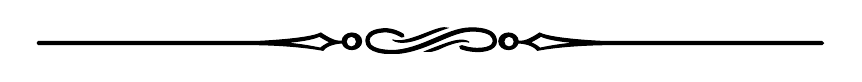
\begin{tikzpicture}
    \node  (C) at (0,0) {};
    \node (D) at (10,0) {};
    \path (C) to [ornament=88] (D);
    \end{tikzpicture}}}}}%
    \end{center}
}

% Title and Author info

\title{Random Kubuntu Stuff\\\large{A descriptive subtitle}}
\author{Julian Tarquin Walsh}
\date{\today}

\newenvironment{boxfig}
    {\begin{center}
    \begin{tabular}{|p{0.9\linewidth}|}
    \hline\\
    }
    {
    \\\\\hline
    \end{tabular}
    \end{center}
    }

\begin{document}

	%%%% Title Page with document information
\pagenumbering{roman}
\maketitle
\sectionline
\tableofcontents
\sectionline
\newpage
\pagenumbering{arabic}

\section{Introduction}

TODO

\section{Marking a File as Executable}
This comes up a bunch in different sections, so I thought it best to include on it's own right at the start. This can be achieved in two ways, the first being to right click on the desired file in the file manager, then click on ``Preferences''. Now check the box next to ``Is executable'', which is shown in \textbf{Figure \ref{fig:executable}}.

\begin{figure}[h]
    \centering
	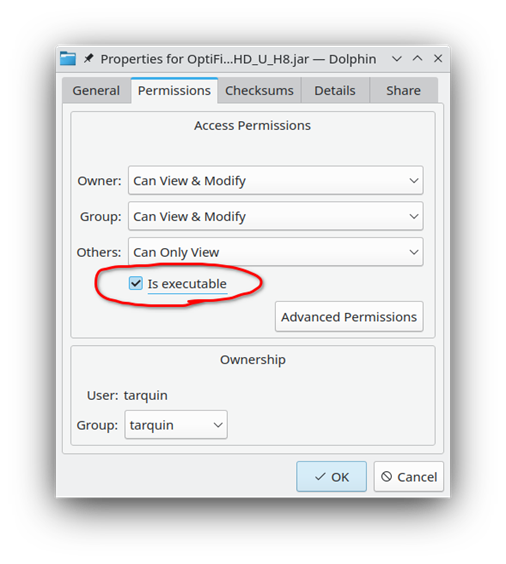
\includegraphics[width=0.5\linewidth]{images/mark_executable}
	\caption{Permissions tab showing the ``Is executable'' checkbox.} \label{fig:executable}
\end{figure}

A file can also be marked as executable from the command line using the \textit{chmod} command.

\begin{lstlisting}
$ chmod +x /path/to/file
\end{lstlisting}

\section{Installing and Manging Software}

\subsection{What's a Package?}

Software on Kubuntu (or any )

\subsection{Updating the System}

\subsubsection{Manually}
Updates can be installed via the ``Discover'' software centre. When updates are available an icon will appear in the system tray, which will open the updates window when clicked. Seen in \textbf{Figure \ref{fig:updates}}.

\begin{figure}[h]
    \centering
    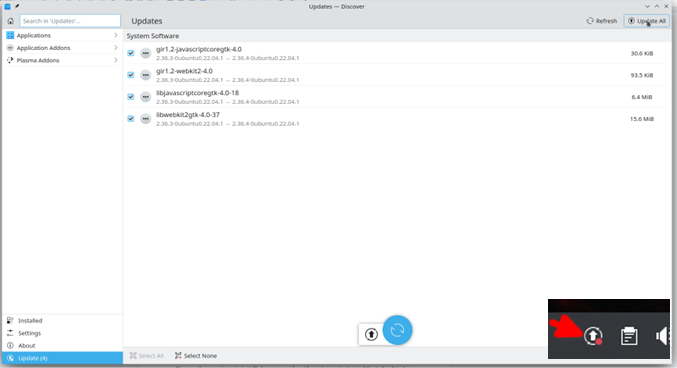
\includegraphics[width=0.6\linewidth]{images/updates}
    \caption{\textit{Main:} The update window of Discover. \textit{Inset:} The update notification icon in the system tray.}\label{fig:updates}
\end{figure}


 To update all packages from the command line, execute the following commands:
\begin{lstlisting}
$ sudo snap refresh
$ sudo apt update
$ sudo apt full-upgrade
\end{lstlisting}

\subsubsection{Using an Update Script}
I find using a script to update the system convenient. Such a script should be placed in a folder called ``bin'' in the user's home folder, since this is automatically added to the path variable, meaning any scripts placed there can be run at the command line from anywhere. The following is (part of) my update script, which is the file \texttt{\$HOME/bin/up}.

\begin{lstlisting}[language=Bash]
#!/bin/bash

set -e  # Causes the script to exit immediately if a command fails

sudo snap refresh
sudo apt update
sudo apt full-upgrade
sudo apt autoremove --purge
sudo apt autoclean

\end{lstlisting}

\section{Misc.}

\subsection{OptiFine}

First, make sure java is installed system wide with \texttt{sudo apt install default-jre}. Then, when double clicking the installer for OptiFine, it will initially display the error in FIG.

\begin{figure}[h]
 \centering
 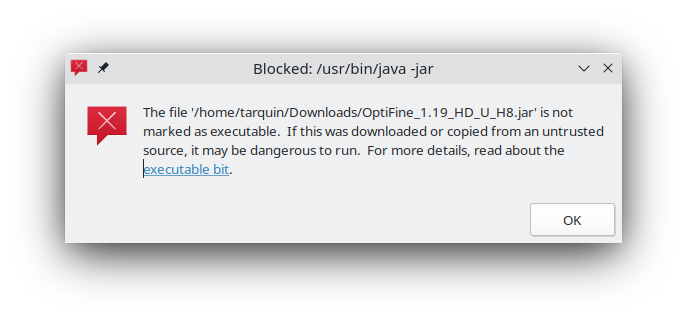
\includegraphics[width=0.6\linewidth]{images/optifine}
 \caption{OptiFine}
\end{figure}

\subsection{The Driver Manager}

If a piece of hardware like a network adapter is not working, the ``Driver Manager'' located in System Settings under ``Hardware'', is a reasonable place to start looking for a solution.

\begin{figure}[h]
 \centering
 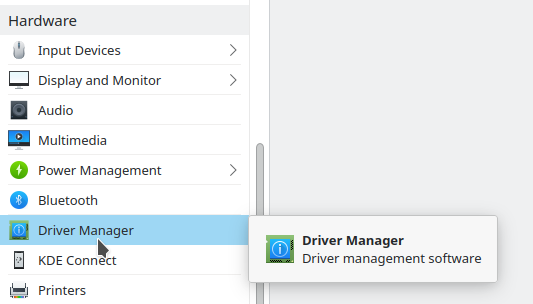
\includegraphics[width=0.6\linewidth]{images/driver_manager_location}
 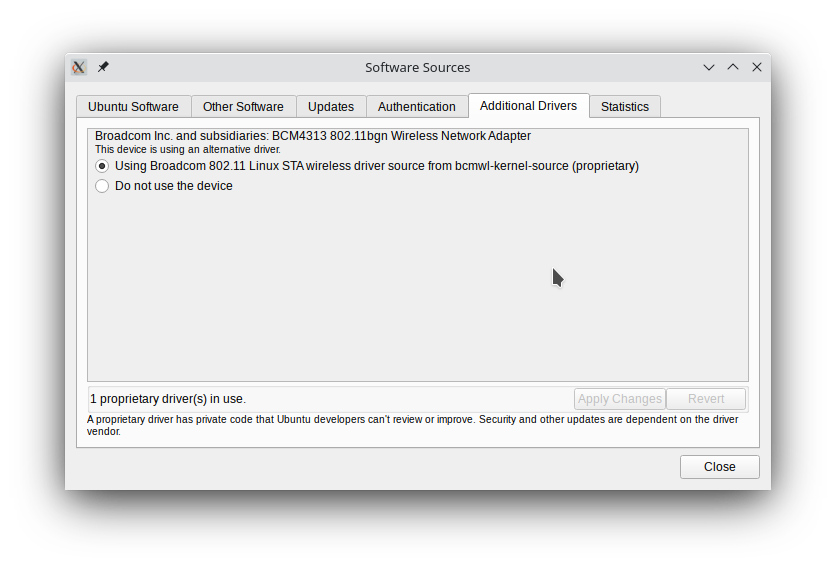
\includegraphics[width=0.6\linewidth]{images/driver_manager_window}
 \caption{\textit{Top:} Location of the Driver Manager system settings module. \textit{Bottom:} The driver manager window.}\label{fig:drivers}
\end{figure}



\subsection{Installing Windows Steam Games}

\subsubsection{Glorius Eggroll}

%\noindent\rule{\linewidth}{0.2ex}
\printbibliography

\end{document}
